\documentclass[aps,prd,twocolumn,showpacs,superscriptaddress,groupedaddress,nofootinbib]{revtex4}  % for review and submission
%\documentclass[aps,preprint,showpacs,superscriptaddress,groupedaddress]{revtex4}  % for double-spaced preprint
\usepackage{graphicx}  % needed for figures
\usepackage{dcolumn}   % needed for some tables
\usepackage{bm}        % for math
\usepackage{amsmath,amssymb}   % for math
\usepackage{color}
\usepackage{float}
\usepackage{multirow}
\usepackage{aas_macros}
\hyphenation{ALPGEN}
\hyphenation{EVTGEN}
\hyphenation{PYTHIA}
\renewcommand{\thefootnote}{\fnsymbol{footnote}}
\newcommand{\mr}{\mathrm}
\newcommand{\mb}{\mathbf}
\renewcommand{\d}{\mathrm{d}}
\newcommand{\e}{\mathrm{e}}
\newcommand{\ii}{\mathrm{i}}
\newcommand{\bea}{\begin{eqnarray}}
\newcommand{\eea}{\end{eqnarray}}
\newcommand{\be}{\begin{equation}}
\newcommand{\ee}{\end{equation}}
\newcommand{\rund}[1]{\left(#1\right)}
\newcommand{\eck}[1]{\left[ #1 \right]}
\newcommand{\bigrund}[1]{\left{#1\right}}
\newcommand{\vc}[1]{\mbox{\boldmath $#1$}}
\newcommand{\dc}{\partial}
\newcommand{\msun}{h^{-1}M_{\odot}}

\def\llabel#1{\label{sc:#1}  {#1}\hspace{0.5cm}}
\def\elabel#1{\label{eq:#1}\fbox{#1}}
%\def\llabel#1{\label{sc:#1}}
%\def\elabel#1{\label{eq:#1}}

% avoids incorrect hyphenation, added Nov/08 by SSR
\hyphenation{ALPGEN}
\hyphenation{EVTGEN}
\hyphenation{PYTHIA}

\begin{document}
% The following information is for internal review, please remove them for submission
\widetext
% the following line is for submission, including submission to the arXiv!!
%\hspace{5.2in} \mbox{Fermilab-Pub-04/xxx-E}

\title{Reconstructing large-scale density field from 3D tidal deformation}

\author{Wen-Kai Hu}
\affiliation{Key Laboratory for Computational Astrophysics,
National Astronomical Observatories, Chinese Academy of Sciences,
20A Datun Road, Beijing 100012, China}
\affiliation{University of Chinese Academy of Sciences, Beijing 100049, China}

\author{Hong-Ming Zhu}
\affiliation{Key Laboratory for Computational Astrophysics,
National Astronomical Observatories, Chinese Academy of Sciences,
20A Datun Road, Beijing 100012, China}
\affiliation{University of Chinese Academy of Sciences, Beijing 100049, China}

\author{Ue-Li Pen}
\affiliation{Canadian Institute for Theoretical Astrophysics, University of Toronto, 60 St. George Street, Toronto, ON M5S 3H8, Canada}
\affiliation{Canadian Institute for Advanced Research, CIFAR Program in Gravitation and Cosmology, Toronto, ON M5G 1Z8, Canada}
\affiliation{Perimeter Institute for Theoretical Physics, 31 Caroline St. N., Waterloo, ON, N2L 2Y5, Canada}
\affiliation{Dunlap Institute for Astronomy and Astrophysics, University of Toronto, 50 St. George Street, Toronto, Ontario M5S 3H4, Canada}

\author{Yu Yu}
\affiliation{Key Laboratory for Research in Galaxies and Cosmology,
Shanghai Astronomical Observatory, Chinese Academy of Sciences,
80 Nandan Road, Shanghai 200030, China}

\author{Xuelei Chen}
\affiliation{Key Laboratory for Computational Astrophysics,
National Astronomical Observatories, Chinese Academy of Sciences,
20A Datun Road, Beijing 100012, China}
\affiliation{Center of High Energy Physics, Peking University, Beijing 100871, China}

\date{\today}

\begin{abstract}
The long-wavelength anisotropic gravitational field can interact with the small-scale density perturbations, leaving an anisotropic distortions on the local power spectrum. The distortions can be used to reconstruct the large-scale density field. In this paper, we develop a 3D tidal reconstruction to reconstruct long-wavelength tidal field from small-scale fluctuations. The 3D reconstruction is better than the 2D method, with higher cross correlation between original matter field and reconstructed $\kappa$ field, lower noise and disappeared anisotropy. We also prove that it is the small-scale fluctuations where the reconstructed large-scale information comes from. Through applying our method to the dark matter field with redshift space distortion (RSD), we find the 3D reconstruction suffers little from the pecular velocity. The 3D reconstruction can be an important addition to the tidal reconstruction.
%applied in many ways, for example, it can recover the long-wavelength modes of the 21cm signal removed in foreground subtraction and measure the redshift-space distortions without sample variance.

\end{abstract}

\pacs{}
\maketitle
%\section{\label{sec:level1}First-level heading}
% sections are not used for PRL papers

\section{Introduction}\label{section:Introduction}
Under the gravitational force, the universe evolves from primordial density perturbations into the structures we see today. The gravitational instability will introduce nonlinear effect and modes will become coupled, which makes information extraction difficult \cite{1999MNRAS.308.1179M}. In Ref. \cite{2012:pen, 2016PhRvD..93j3504Z}, a powerful tool named cosmic tidal reconstruction has been developed. By using the small-scale non-Gaussianity induced by tidal field, they originates a new method for the reconstruction of large-scale structures. The evolution of small-scale fluctuation $\delta(\bm{k}_{s})$ is influenced by the long-wavelength gravitational potential $\Phi_{L}$, this results in isotropic and anisotropic distortion on the local small-scale power spectrum. We can use this mode coupling to reconstruct the large-scale density field from the small-scale fluctuations. Since many other processes can result in isotropic distortions on the local small-scale power spectrum, the anisotropic distortions are more powerful to reconstruct the large-scale structure. Using the quadratic estimators, the long-wavelength tidal field can be reconstructed.

The tidal field can be decomposed into five independent components: $\gamma_{1}$, $\gamma_{2}$, $\gamma_{x}$, $\gamma_{y}$ and $\gamma_{z}$. Same as the gravitational lensing, these components describe how a density field changes its shape under the influence of the gravitational force. Due to the analogous physical process, the tidal shear reconstruction is similar to the reconsruction in gavitational lensing. In the previous work\cite{2012:pen,2016PhRvD..93j3504Z}, the tidal reconstruction has been exploited, and encouraging results are obtained. However, the former work only takes two transverse shear terms $\gamma_{1}$ and $\gamma_{2}$ into consideration, the fluctuations of long-wavelength density field along the line of sight (LOS) has to be estimated by the change of the two transverse components along the LOS. In this paper, we use all 5 shear terms to reconstruct the large-scale density field. The reconstructed density field from the updated method has lower noise, better isotropy and higher correlation with the original dark matter field. Besides, our method can reconstruct the large-scale density field very well even only with limited fluctuation modes from the small-scale structures (see Sec. \ref{section:Simulations}).

Different with the reconstruction with transverse shape tensor, the tangential shape tensor will be affected by RSD. However, we find that the benefits we gain from the 3D reconstruction can overtake the disadvantage introduced by RSD (see Sec. \ref{section:Simulations}).

In Sec. \ref{section:Tidal Reconstruction}, we deduce the estimate of the large-scale density field. In Sec. \ref{section:Simulations}, we introduce the reconstruction algorithm and study the performance of it with dark matter density fields from $N$-body simulations. In Sec. \ref{section:Discussion}, the fine details of 3D tidal reconstruction method will be discussed. In Sec. \ref{section:Conclusion}, we give a conclusion for this study.

\section{Tidal Reconstruction}\label{section:Tidal Reconstruction}
In this section we give a brief description of the physical process of the tidal interaction, then we construct the estimators for tidal shear fields.

The anisotropic gravitational force arising from long-wavelength tidal field will change the way the dark matter fluid element moves. Then from the the equation of motion, we can obtain the coupling between the long-wavelength tidal field and the small-scale density fluctuations \cite{2016PhRvD..93j3504Z}.

The local small-scale power spectrum under the distortion from the tidal field can be described as \cite{2016PhRvD..93j3504Z}:

\begin{equation}
P(\bm{k},\tau)|_{t_{ij}} = P_{1s}(k,\tau)+\hat{k}^i\hat{k}^jt_{ij}^{(0)}P_{1s}(k,\tau)f(k,\tau),
\label{eq1}
\end{equation}
where 
\begin{equation}
f(k,\tau) = 2\alpha(\tau) - \beta(\tau)\frac{d\mathrm{ln}P_{1s}(k,\tau)}{d\mathrm{ln}k},
\label{eq2}
\end{equation}
$P_{1s}(k,\tau)$ is the small-scale power spectrum and $t^{(0)}_{ij}$ refers to the tidal field at initial time,  $\alpha(\tau) = -D_{\sigma1}(\tau) + F(\tau)$ and $\beta(\tau) = F(\tau)$, 

\begin{equation}
D_{\sigma1}(\tau) = \int_{0}^{\tau}d\tau'\frac{H(\tau)D(\tau') - H(\tau')D(\tau)}{\dot{H}(\tau')D(\tau') - H(\tau')\dot{D}(\tau')}\frac{T(\tau')D{(\tau')}}{D(\tau)},
\label{eq3}
\end{equation}

\begin{equation}
F(\tau)=\int_{0}^{\tau}d\tau''a(\tau'')T(\tau'')G(\tau-\tau''),
\label{eq4}
\end{equation}
$G(\tau -\tau'')=\int_{\tau''}^{\tau}d\tau'/a(\tau')$, $T(\tau) = D(\tau)/a(\tau)$, $a(\tau)$ is the scale factor, $H(\tau)$ denotes the Hubble parameter and $D(\tau)$ is the linear growth function. 

Eq. (\ref{eq1}) illustrates the interaction between the small-scale fluctuations and the long-wavelength tidal field. There are two points on which we should lay much emphasis. 
Firstly, we use the linear assumption when we deduce the density fluctuation, but the assumption holds badly in the small scales where nonlinear effect dominants. So our reconstruction will work badly in highly nonlinear scales. Secondly, the description above only includes the leading-order coupling between the small-scale density fluctuations and the long-wavelength tidal field. However, there are many more higher-order coupling modes in the tidal interactions. Our reconstruction may misestimate the nonlinear coupling and lead to a bias between our tidal shear estimators and the real tidal fields.

%\section{Tidal Shear Estimators}

The tidal symmetric tensor $t_{ij}$ can be decomposed as $t_{ij} = \Phi_{L,ij} - \delta_{ij}\nabla^{2}\Phi_{L}/3$, and \cite{1973gw, 2012:jeong}: 

\begin{eqnarray}
t_{ij}=\left( \begin{array}{ccc}
\gamma_{1}-\gamma_{z} & \gamma_{2} & \gamma_{x}\\
\gamma_{2} & -\gamma_{1}-\gamma_{z} & \gamma_{y}\\
\gamma_{x} & \gamma_{y} & 2\gamma_z
\end{array} \right),
\label{eq5}
\end{eqnarray}
where $\gamma_{1}=(\Phi_{L,11}-\Phi_{L,22})/2$, $\gamma_{2}=\Phi_{L,12}$, $\gamma_{x}=\Phi_{L,13}$, $\gamma_{y}=\Phi_{L,23}$, and $\gamma_{z}=(2\Phi_{L,33}-\Phi_{L,11}-\Phi_{L,22})/6$.
The $t_{ij}$ here is decomposed along the $\hat{z}$ direction, and there are still two more directions along which we can carry out the decomposition. In order to express clearly, we only discuss the decomposition along the $\hat{z}$ direction from here on. We will show it doesn't matter which axis acts as a special direction in a moment.

With the orthogonal components we get above, Eq. (\ref{eq1}) can be written as
\begin{eqnarray}
P(\bm{k},\tau)|_{t_{ij}}&=&P_{1s}(k,\tau)+
[(\hat{k}_1^2-\hat{k}_2^2)\gamma_1^{(0)}+
2\hat{k}_1\hat{k}_2\gamma_2^{(0)}+\nonumber\\
&&2\hat{k}_1\hat{k}_3\gamma_x^{(0)}+
2\hat{k}_2\hat{k}_3\gamma_y^{(0)}+
(2\hat{k}_3^2-\hat{k}_1^2-\hat{k}_2^2)\gamma_z^{(0)}]
\nonumber\\&&\times P_{1s}(k,\tau)f(k,\tau).
\label{eq6}
\end{eqnarray}

In Refs. \cite{2012:pen, 2016PhRvD..93j3504Z} the tidal shear estimators $\gamma_{1}$ and $\gamma_{2}$  have been deduced, but only the tidal shear fields in the tangential plane are used directly. We can construct the tidal shear estimators with all 5 components in the tidal tensor $t_{ij}$, taking fluctuation modes from all directions into consideration.

Before we compute the estimators for the tidal shear fields, we apply a Gaussianization technique \cite{1992MNRAS.254..315W} to the original dark matter field to reduce non-Gaussianity. This technique reassigns the pixel densities with a Gaussian probability distribution, and the order of the pixel densities remains to be unchanged.
Under the Gaussian assumption and long-wavelength limit, through the method of maximum likelihood \cite{2008:lu} or inverse variance weighting \cite{2010lu,2012bucher}, the unbiased minimum variance quadratic estimators can be deduced: 
\begin{equation}
\begin{split}
&\hat{\gamma}_1=\frac{1}{Q}\int\frac{d^3k}{(2{\pi})^3}\frac{|\delta_{g}(\bm{k})|^2}{L^3}\frac{P(k)}{P^2_{tot}(k)}f(k)(\hat{k}^2_{1}-\hat{k}^2_{2}),\\
&\hat{\gamma}_2=\frac{1}{Q}\int\frac{d^3k}{(2{\pi})^3}\frac{|\delta_{g}(\bm{k})|^2}{L^3}\frac{P(k)}{P^2_{tot}(k)}f(k)(2\hat{k}_{1}\hat{k}_{2}),\\
&\hat{\gamma}_x=\frac{1}{Q}\int\frac{d^3k}{(2{\pi})^3}\frac{|\delta_{g}(\bm{k})|^2}{L^3}\frac{P(k)}{P^2_{tot}(k)}f(k)(2\hat{k}_{1}\hat{k}_{3}),\\
&\hat{\gamma}_y=\frac{1}{Q}\int\frac{d^3k}{(2{\pi})^3}\frac{|\delta_{g}(\bm{k})|^2}{L^3}\frac{P(k)}{P^2_{tot}(k)}f(k)(2\hat{k}_{2}\hat{k}_{3}),\\
&\hat{\gamma}_z=\frac{1}{Q}\int\frac{d^3k}{(2{\pi})^3}\frac{|\delta_{g}(\bm{k})|^2}{L^3}\frac{P(k)}{P^2_{tot}(k)}f(k) \\
&\quad\quad\times[2\hat{k}^2_{3}-\hat{k}^2_{1}-\hat{k}^2_{2}]/3,
\end{split}
\label{eq7}
\end{equation}
where $P_{tot}(k) = P(k) + P_{N}(k)$, $P_{N}(k)$ is the noise spectrum, $\delta_{g}$ is the Gaussianized $1+\delta_{1s}$, $\delta_{1s}$ refers to the small-scale fluctuations, and
%\begin{equation}
%\begin{split}
%&Q_{\gamma_1}=\int\frac{d^3k}{(2{\pi})^3}\frac{P^2(k)}{P^2_{tot}(k)}f^2(k)(\hat{k}^2_{1}-\hat{k}^2_{2})^2,\\
%&Q_{\gamma_2}=\int\frac{d^3k}{(2{\pi})^3}\frac{P^2(k)}{P^2_{tot}(k)}f^2(k)(2\hat{k}_{1}\hat{k}_{2})^2,\\
%&Q_{\gamma_x}=\int\frac{d^3k}{(2{\pi})^3}\frac{P^2(k)}{P^2_{tot}(k)}f^2(k)(2\hat{k}_{1}\hat{k}_{3})^2,\\
%&Q_{\gamma_y}=\int\frac{d^3k}{(2{\pi})^3}\frac{P^2(k)}{P^2_{tot}(k)}f^2(k)(2\hat{k}_{2}\hat{k}_{3})^2,\\
%&Q_{\gamma_z}=\int\frac{d^3k}{(2{\pi})^3}\frac{P^2(k)}{P^2_{tot}(k)}f^2(k)([2\hat{k}^2_{3}-\hat{k}^2_{1}-\hat{k}^2_{2}]/3)^2
%\end{split}
%\label{eq8}
%\end{equation}
%If we integrate them over angles in the Fourier space we will get that $Q_{\gamma_1} = Q_{\gamma_2} = Q_{\gamma_x} = Q_{\gamma_y} = Q_{\gamma_z} = Q,$
\begin{equation}
Q = \int\frac{2k^2dk}{15\pi^2}\frac{P^2(k)}{P^2_{tot}(k)}f^2(k).
\label{eq9}
\end{equation}
By using Parseval's theorem, in real space, we can present the quadratic estimators as:
\begin{equation}
\begin{split}
&\hat{\gamma}_1=\frac{1}{L^3}\int d^3x[\delta^{w_{1}}_{g}(\bm{x})\delta^{w_{1}}_{g}(\bm{x})-\delta^{w_{2}}_{g}(\bm{x})\delta^{w_{2}}_{g}(\bm{x})],\\
&\hat{\gamma}_2=\frac{1}{L^3}\int d^3x[2\delta^{w_{1}}_{g}(\bm{x})\delta^{w_{2}}_{g}(\bm{x})],\\
&\hat{\gamma}_x=\frac{1}{L^3}\int d^3x[2\delta^{w_{1}}_{g}(\bm{x})\delta^{w_{3}}_{g}(\bm{x})],\\
&\hat{\gamma}_y=\frac{1}{L^3}\int d^3x[2\delta^{w_{2}}_{g}(\bm{x})\delta^{w_{3}}_{g}(\bm{x})],\\
&\hat{\gamma}_z=\frac{1}{L^3}\int d^3x[2\delta^{w_{3}}_{g}(\bm{x})\delta^{w_{3}}_{g}(\bm{x})-\delta^{w_{1}}_{g}(\bm{x})\delta^{w_{1}}_{g}(\bm{x})-\\
&\quad\quad\delta^{w_{2}}_{g}(\bm{x})\delta^{w_{2}}_{g}(\bm{x})]/3
\end{split}
\label{eq10}
\end{equation}
where 
\begin{eqnarray}
\delta^{w_{i}}_{g}(\bm{k}) = \delta_{g}(\bm{k})w_{i}(\bm{k}),
\label{eq11}
\end{eqnarray}
and
\begin{eqnarray}
w_{i}(\bm{k}) = \left[\frac{P(k)f(k)}{QP^2_{tot}(k)}\right]^{1/2}i\hat{k}_{i}.
\label{eq12}
\end{eqnarray}
In the long-wavelength limit that the tidal shear fields vary slowly in the space $L^3$, the unbiased minimum variance estimators of tidal fields can be simplified as: 

\begin{equation}
\begin{split}
&\hat{\gamma}_1(\bm{x})=\big[{\delta}^{w_1}_g(\bm{x}){\delta}^{w_1}_g(\bm{x})-
{\delta}^{w_2}_g(\bm{x}){\delta}^{w_2}_g(\bm{x})\big],\\
&\hat{\gamma}_2(\bm{x})=\big[2{\delta}^{w_1}_g(\bm{x}){\delta}^{w_2}_g(\bm{x})\big],\\
&\hat{\gamma}_x(\bm{x})=\big[2{\delta}^{w_1}_g(\bm{x}){\delta}^{w_3}_g(\bm{x})\big],\\
&\hat{\gamma}_y(\bm{x})=\big[2{\delta}^{w_2}_g(\bm{x}){\delta}^{w_3}_g(\bm{x})\big],\\
&\hat{\gamma}_z(\bm{x})=\big[2{\delta}^{w_3}_g(\bm{x}){\delta}^{w_3}_g(\bm{x})-
{\delta}^{w_1}_g(\bm{x}){\delta}^{w_1}_g(\bm{x}) \\
&\quad\quad\quad-{\delta}^{w_2}_g(\bm{x}){\delta}^{w_2}_g(\bm{x})\big]/3.
\end{split}
\label{eq13}
\end{equation}
We can obtain the convergence field $\kappa \equiv \nabla^2\Phi_L/3$ from the tidal shear fields:
%the trace part of this traceless tensor is given by 
%$\nabla^2\Phi_L=3K_{ij}t_{ij}/2\sim\delta_L$, where $K_{ij}=\partial_i\partial_j/\nabla^2$. Thus we get the estimator for the large scale density from these five tidal shear fields. In Fourier space, we have,
\begin{eqnarray}
\kappa(\bm{k})&=&\frac{1}{2k^2}
[(k_1^2-k_2^2)\gamma_1(\bm{k})+2k_1k_2\gamma_2(\bm{k})+2k_1k_3\gamma_x(\bm{k})\nonumber\\
&&+2k_2k_3\gamma_y(\bm{k})+(2k_3^2-k_1^2-k_2^2)\gamma_z(\bm{k})],
\label{eq14}
\end{eqnarray}
where $k^2 = k_1^2+k_2^2+k_3^2$.

Same as the decomposition of $t_{ij}$, $\kappa$ also has another two ways to decompose. Combining the expression of the $\gamma$ and $\kappa$, it shows that no matter along which direction we decompose, we will get the same isotropic $\kappa$. However, when the dark matter field is affected by RSD, the line of sight will be a special direction, and different decomposition will have different reconstruction results.
For simplicity, we will just use the way that uses the ${\hat{z}}$ as the decomposition direction and the LOS in the rest of the paper.

%=======================================

\section{Simulations}\label{section:Simulations}
In this section we show the algorithm of the reconstruction. Then we perform reconstruction with various smoothing scales and different information sources to test our method. After that, we compare the reconstruction with different combinations of $\gamma$ fields. Finally, we give a simple description of the influence induced by RSD effect.

Our analysis is on the foundation of high-resolution $N$-body simulations with the CUBEP$^3$M code \cite{2013MNRAS.436..540H}, it contains $2048^3$ dark matter particles in a box with side length equal to 1.2Gpc/$h$. We conduct the simulation with $\Omega_{b}=0.049$, $\Omega_{c}=0.259$, $h=0.678$, $A_{s}=2.139\times10^{-9}$ and $n_{s}=0.968$. To obtain a better statistic quality, we generated ten fields with independent initial conditions.

\subsection{Reconstruction algorithm}

We apply the following algorithm to carry out the reconstrction:

(1) We smooth the field with a Gaussian window $W(\bm{r}) = e^{-\bm{r}^2/2R^2}$. Then we apply a Gaussianization technique to the smoothed dark matter field. 

(2) After that, we multiply the field with the filter $w_{i}(\bm{k})$ as what we have showed in Eq. (\ref{eq11}) and Eq. (\ref{eq12}). Applying the Eq. (\ref{eq13}), the tidal shear fields $\gamma_{1}$, $\gamma_{2}$, $\gamma_{x}$, $\gamma_{y}$ and $\gamma_{z}$ can be obtianed.

(3) Then, we use these five estimators to generate the convergence field $\kappa(\bm{k})$ according to Eq. (\ref{eq14}). 

To minimize the noise in the reconstructed field and correct the bias between the $\kappa$ field and the original dark matter field, we will apply a Wiener filter to $\kappa$ and devide the field by a bias factor.

The reconstructed noisy $\kappa$ field could be expressed as:
\begin{eqnarray}
\kappa(k_\perp, k_\parallel) = b(k_\perp, k_\parallel)
\delta_L(k_\perp, k_\parallel) + n(k_\perp, k_\parallel),
\label{eq17}
\end{eqnarray}
where $b(k_\perp, k_\parallel)$ is the bias factor and $n(k_\perp,k_\parallel)$
is the noise in the reconstructed $\kappa$ field.
Through the cross correlation of $\kappa$ and $\delta$ and the auto correlation of $\kappa$ and $\delta$, the bias and noise can be computed,

\begin{eqnarray}
\langle\kappa\delta\rangle = b\langle\delta\delta\rangle,
\label{eq18}
\end{eqnarray}

\begin{eqnarray}
\langle\kappa\kappa\rangle = b^2\langle\delta\delta\rangle+\langle nn\rangle,
\label{eq19}
\end{eqnarray}
So,
\begin{eqnarray}
b(k_\perp, k_\parallel) = \frac{P_{\kappa\delta}(k_\perp, k_\parallel)}{P_{\delta}(k_\perp, k_\parallel)},
\label{eq20}
\end{eqnarray}
and 
\begin{eqnarray}
P_{n}(k_\perp, k_\parallel) = P_{\kappa}(k_\perp, k_\parallel) - b^2(k_\perp, k_\parallel)P_{\delta}(k_\perp, k_\parallel).
\label{eq21}
\end{eqnarray}
Then the unbiased reconstructed clean field $\kappa$ can be obtained by:
\begin{eqnarray}
\hat{\kappa}(k_\perp, k_\parallel) = \frac{\kappa(k_\perp, k_\parallel)}{b(k_\perp, k_\parallel)}W(k_\perp, k_\parallel),
\label{eq22}
\end{eqnarray}
where the $W(k_\perp, k_\parallel)$ is the Wiener filter and 
\begin{eqnarray}
W(k_\perp, k_\parallel) = \frac{P_{\delta}(k_\perp, k_\parallel)}{P_{\delta}(k_\perp, k_\parallel) + P_{n}(k_\perp, k_\parallel)/b^2(k_\perp, k_\parallel)}.
\label{eq23}
\end{eqnarray}
After the Fourier tansformation of $\hat{\kappa}(\bm{k})$, we can obtain the optimal estimate of the large-scale density field. 

%=======================================

\subsection{Results}

%\subsection{Bias of Estimator}
We use the algorithm described above to reconstruct large-scale density field with different smoothing scales. Figure. \ref{1D_bias_smooth} illustrates the bias between our $\kappa$ field and the original dark matter fields. The bias is defined as $b(k) = P_{\kappa\delta}(k)/P_{\delta}(k)$. The error bars are estimated using the bootstrap method, so do the error in the other figures below.  Except for the reconstruction without smoothing, the bias is nearly constant at the large scales, indicating the reconstructed $\kappa$ field can be a good estimate of the original dark matter field. The bias drops to zero at the small scales, since our reconstruction doesn't model the nonlinear process at those scales and the results from small scales are not reliable.

\begin{figure}[h!]
     \centering
     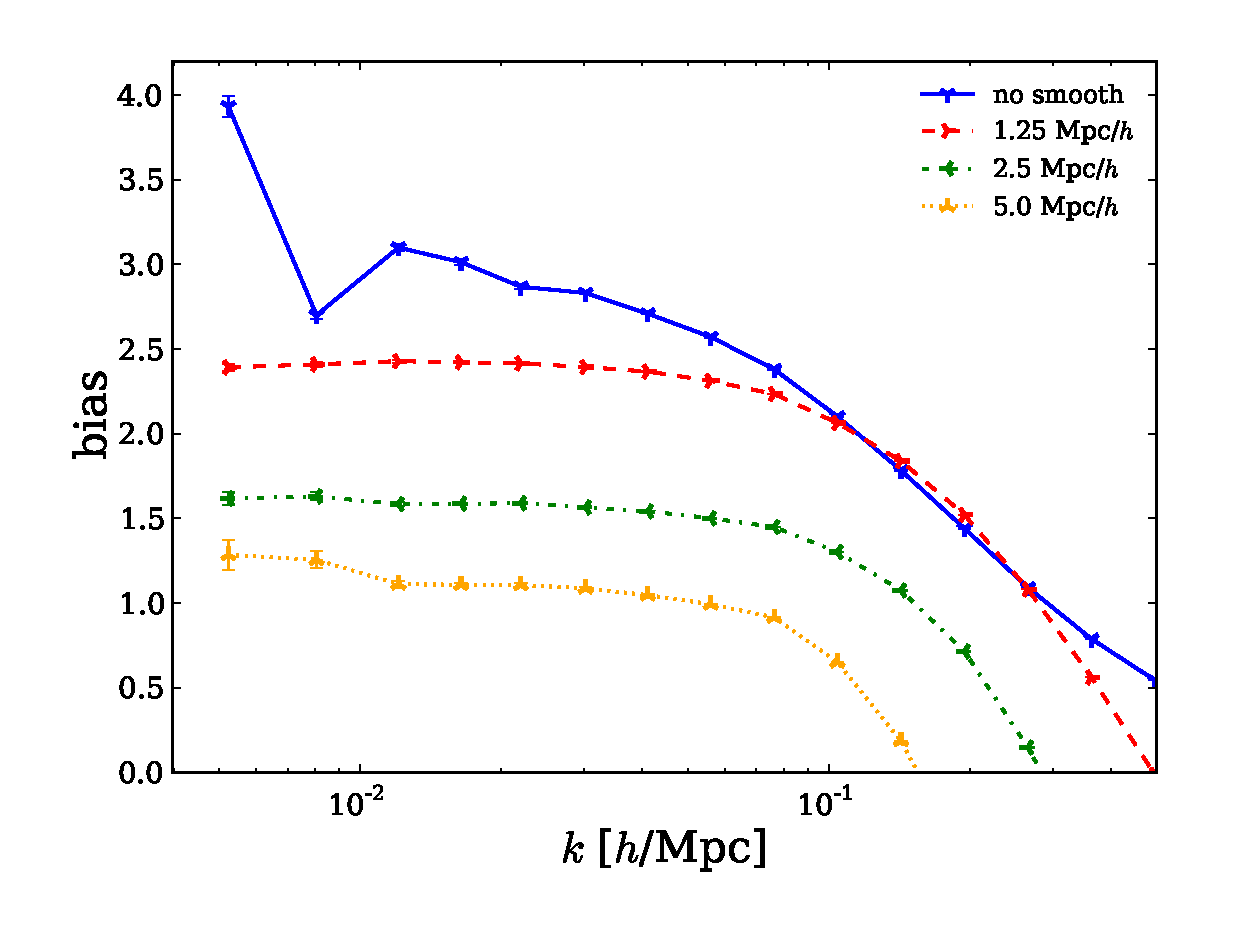
\includegraphics[width=9cm]{1D_bias_smooth.eps}
     \caption{The bias, which is defined as $b(k) = P_{\kappa\delta}(k)/P_{\delta}(k)$, from reconstruction with different smoothing scales: no smoothing, $R$ = 1.25, 2.5 and 5.0 Mpc/$h$.}
     \label{1D_bias_smooth}
\end{figure}

%\subsection{Noise of Reconstruction}
\begin{figure}[h!]
     \centering
     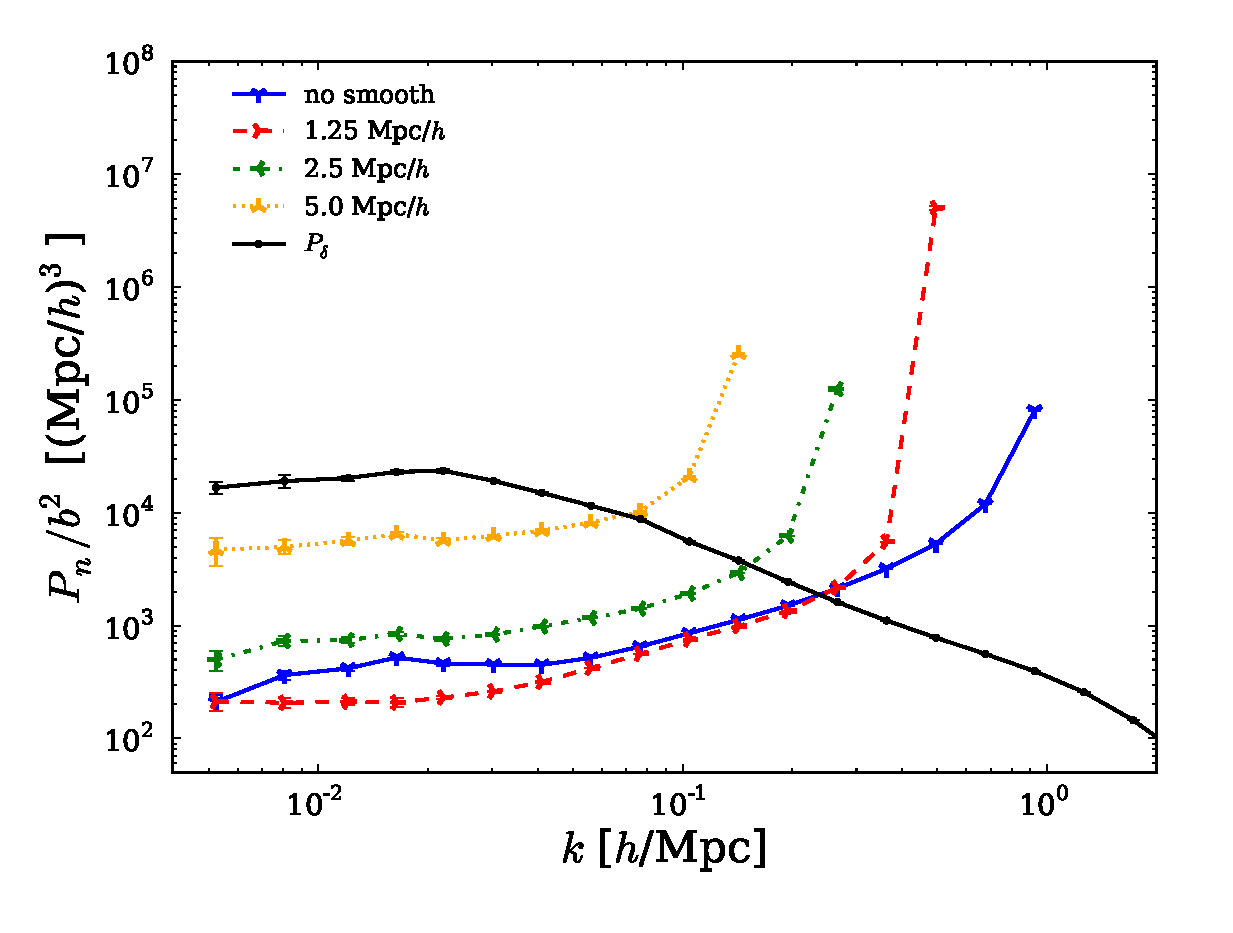
\includegraphics[width=9cm]{1D_noise_bias_smooth.eps}
     %\includegraphics[width=9cm]{1D_noise_bias_cut.eps}
     \caption{The noise, which is defined as  $P_{n}(k)/b^2(k)$, from reconstruction with different smoothing scales: no smoothing, $R$ = 1.25, 2.5 and 5.0 Mpc/$h$. For comparison we plot the $P_{\delta}(k)$ with the noise together.}
     \label{1D_noise_bias}
     \end{figure}

We show the noise of the reconstructed $\kappa$ field from the reconstruction with different smoothing scales in Fig. \ref{1D_noise_bias}. The noise is computed as $P_{n}(k)/b^2(k)$, where $P_{n}(k) = P_{\kappa}(k) - b^2(k)P_{\delta}(k)$.  According to Fig. \ref{1D_noise_bias}, all of the noise spectra are lower and flatter at the large scales, however, blow up at the small scales. With smoothing scales getting larger the amplitude of the noise becomes higher and the scale where the noise starts to blow up moves to smaller $k$.

\begin{figure}[h!]
     \centering
     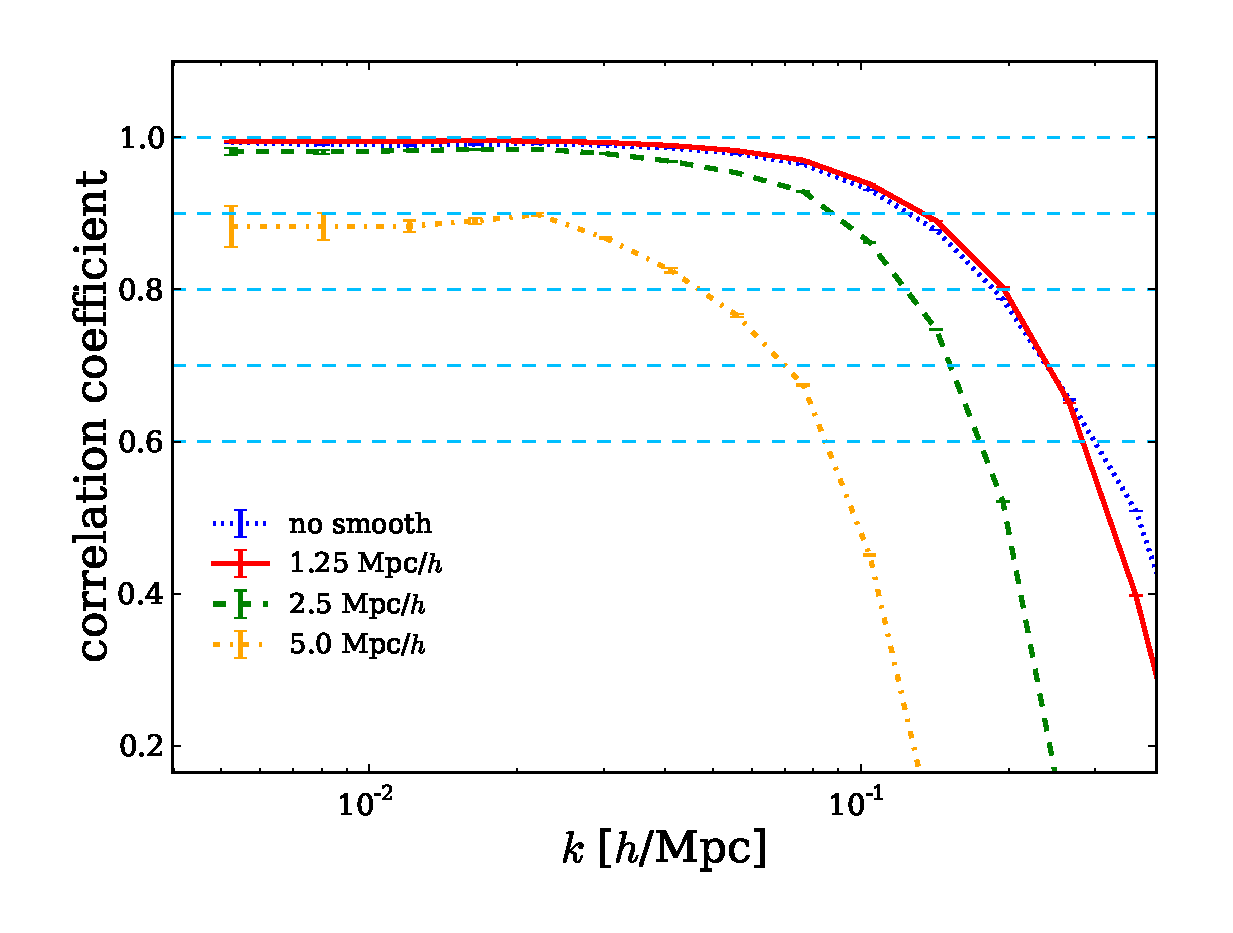
\includegraphics[width=9cm]{1D_correlation_aver_smooth.eps}
     \caption{The correlation coefficients of reconstructions with different smoothing scales: no smoothing, $R$ = 1.25, 2.5 and 5.0 Mpc/$h$. }
     \label{1D_correlation_aver_smooth}
\end{figure}

%\subsection{Effect of smoothing scale}
In Fig. \ref{1D_correlation_aver_smooth}, we present correlation coefficients from reconstructions with different smoothing scales, defined as:

\begin{eqnarray}
r(k) = \frac{P_{\delta\kappa}(k)}{\sqrt{P_{\delta}(k)P_{\kappa}(k)}} = \frac{1}{\sqrt{1+\eta(k)}},
\label{correlation}
\end{eqnarray}
where $\eta$ = $P_{n}/(b^{2}P_{\delta})$, and $P_{n}$ refers to the noise spectrum, $b$ is the bias.
We can see that all of the reconstructions have pretty good correlation. With the smoothing scale becoming larger, the correlation coefficients get lower, the errors increase and the de-correlation scales move to larger scales.

%From the Fig. \ref{1D_noise_bias} and Fig. \ref{1D_correlation_aver_smooth}, it is obvious that larger noise will make the reconstruction worse. Eq. (\ref{correlation}) has showed that it is the relative amplitude of the noise and the signal we want ($b^2P_{\delta}$) affect the results of the reconstruction.
Our reconstruction makes use of the small-scale fluctuations induced by the long-wavelength tidal field to reconstruct the large-scale density field. However, the strong self-gravitational interactions at the small scales will dominate over the weak gravitational interactions with the tidal field. A proper scale smoothing can reduce nonlinear effects. While larger-scale smoothing leaves less small-scale structure modes to be used to reconstruct the large-scale density field. Then the reconstructed field will contain more noise. According to the results we show above, the reconstruction with 1.25 Mpc/$h$ smoothing is optimal. We will use 1.25 Mpc/$h$ smoothing in the reconstruction in the rest of this paper except other noted. 

In Fig. \ref{1Dspec_dm} we show the auto and cross power spectrum of the dark matter density field and the $\kappa$ field obtained from the reconstruction with 1.25 Mpc/$h$ smoothing. At the scales between 0.005$h$/Mpc $< k <$ 0.1$h$/Mpc, there is fairly good accordance between the original density field and the reconstructed $\kappa$ field. And at the smaller scale, the correlation between $\delta$ and $\kappa$ goes down quickly, due to the physical process at those small scales is not modeled explicitly in our reconstruction. We are not able to reconstruct the structures at small scales very well.

\begin{figure}[h!]
     \centering
     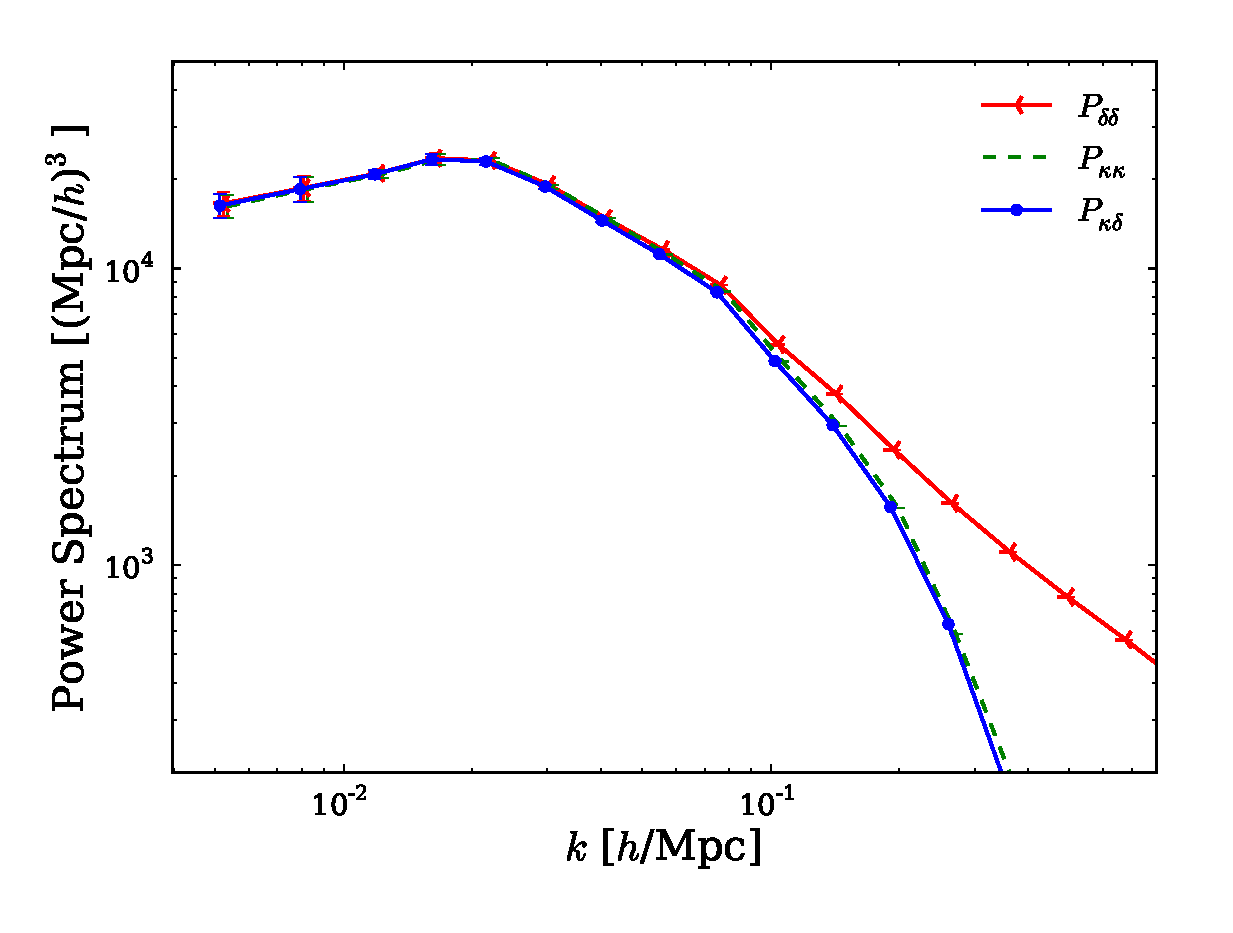
\includegraphics[width=9cm]{1Dspec_dm.eps}
     \caption{The auto-spectra and cross-spectrum of initial density field and $\kappa$ field. To display clearly, we shift these points a little.}
     \label{1Dspec_dm}
\end{figure}

\begin{figure}[!htp]
      \centering
      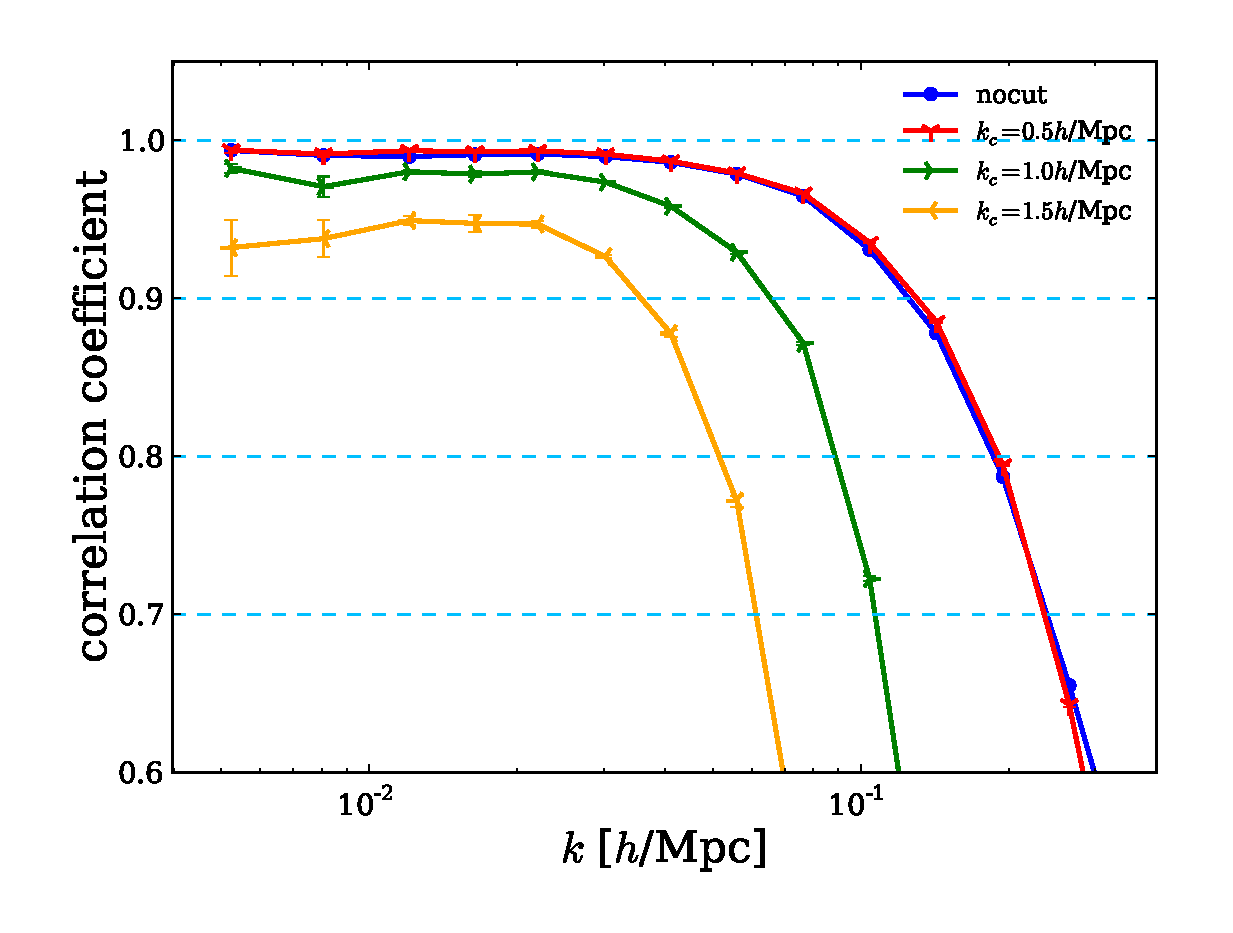
\includegraphics[width=9cm]{1D_correlation_aver_cut.eps}
      \caption{Correlation coefficients from reconstruction with dark matter field undergoes $k$ = 0.5$h$/Mpc, 1.0$h$/Mpc and 1.5$h$/Mpc cutting.}
      \label{1D_correlation_aver_cut}
\end{figure}

\subsection{Test of independence}
So far, we have developed a powerful method to reconstruct the large-scale structure and obtain excellent results. However, there is always a doubt that whether the reconstructed large-scale density field is from the small-scale fluctuations in the original dark matter field, or just from the large scales of the original field. To verify this, in the the original dark matter fields, we remove the fluctuation modes in the region where $k$ smaller than 0.5$h$/Mpc, 1.0$h$/Mpc and 1.5$h$/Mpc respectively. Then we reconstrcut the large-scale density field with these processed fields. In these reconstructions, we skip the process of smoothing to get rid of the influence induced by smoothing. We show the results in Fig. \ref{1D_correlation_aver_cut}.

Figure. \ref{1D_correlation_aver_cut} points out that our reconstruction performs very well even we remove the modes from $k$ smaller than 1.5$h$/Mpc. And it is obvious that more small-scale fluctuation modes being removed makes the reconstruction worse. So, we prove that when recovering the large-scale density field, it is the small-scales fluctuations from the original field that our method makes use of.

\subsection{Different combinations of shear fields}

\begin{figure*}[!htp]
     \centering
     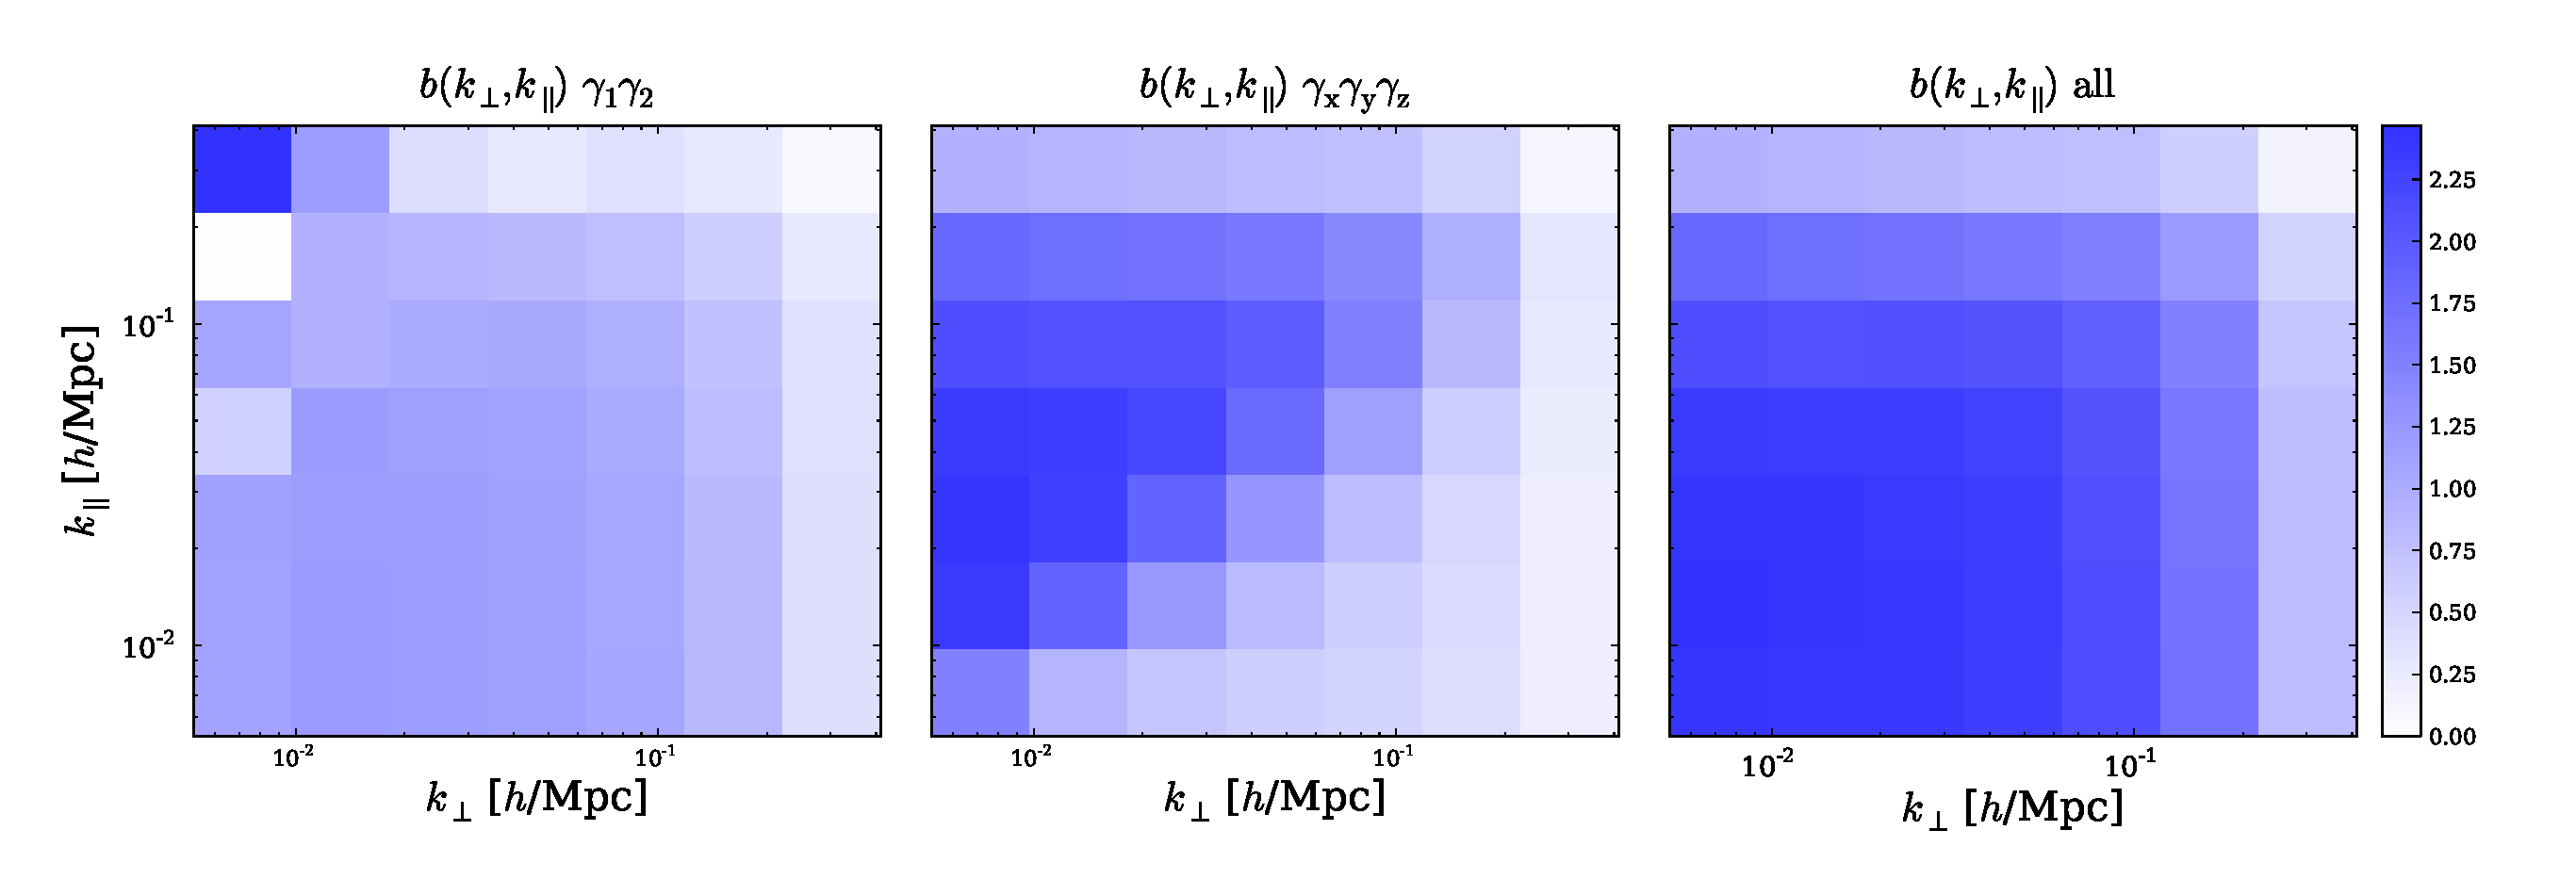
\includegraphics[width=18cm]{bias_subfigure.eps}
     %\includegraphics[width=9cm]{bias.eps}
     \caption{The 2D bias factor. The upper panel shows the 2D reconstruction's result, the central panel shows results from the reconstruction with $\gamma_{x}$, $\gamma_{y}$ and $\gamma_{z}$, and the lowest panel shows the 3D result. Some points saturate in the left corner in upper panel, which are not reliable.}
     \label{2Dbias}
\end{figure*}

\begin{figure}[!htp]
     \centering
     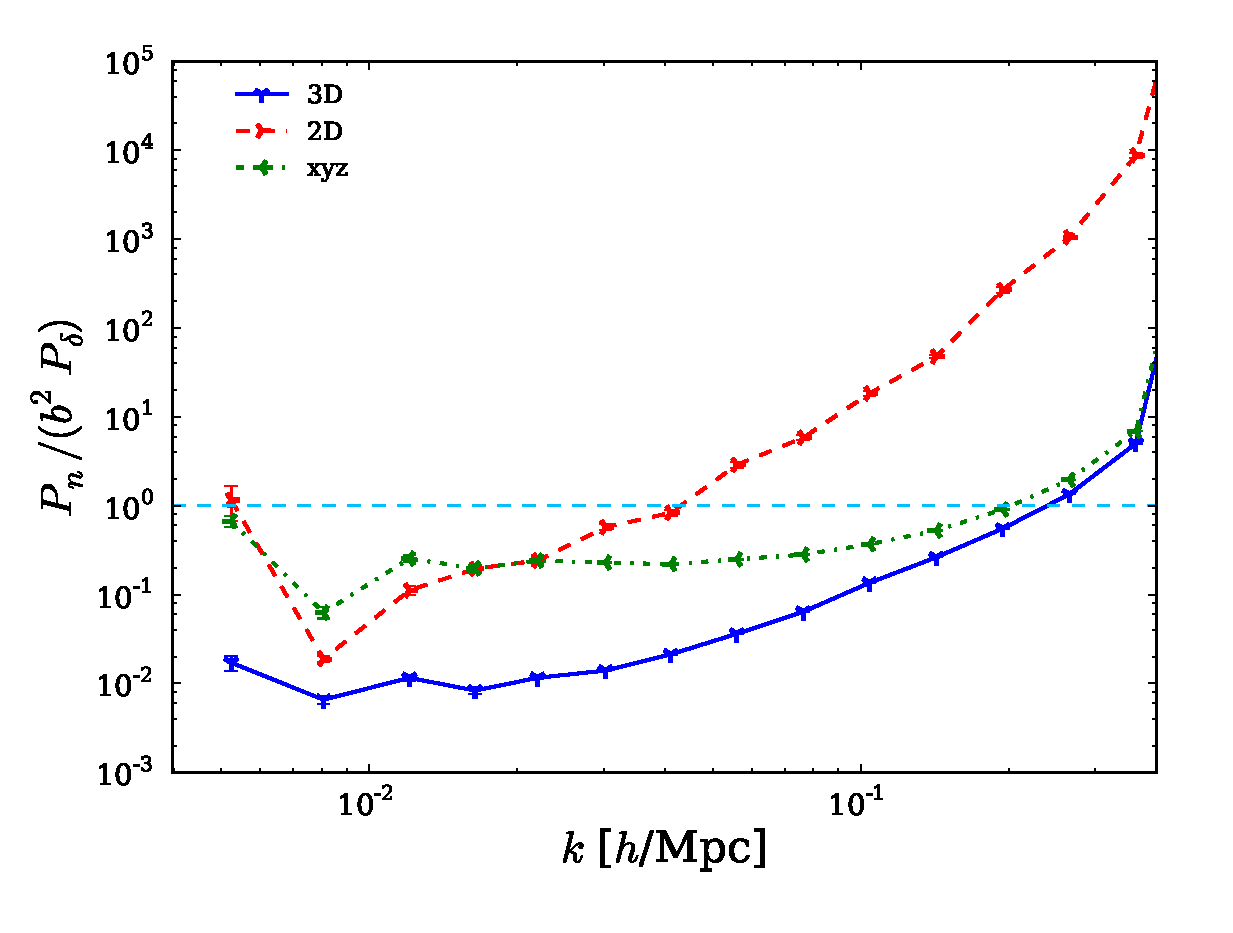
\includegraphics[width=9cm]{1D_noise_bias_all.eps}
     \caption{The noise power spectrum, which is defined as $P_{n}(k)/(b^2(k)P_{\delta(k)})$, from three different ways of tidal reconstruction.}
     \label{1Dnoise}
     \end{figure}

\begin{figure}[h!]
     \centering
     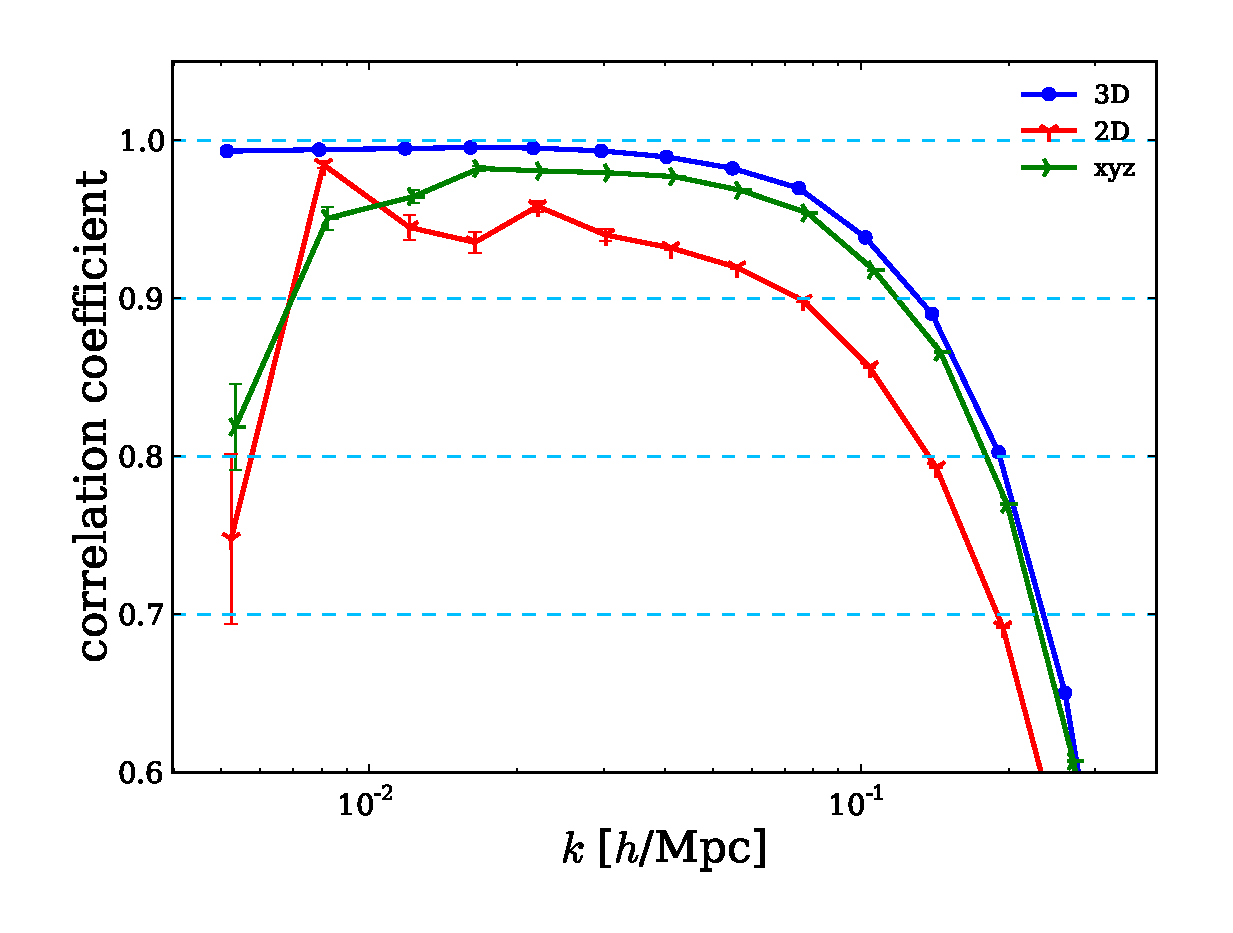
\includegraphics[width=9cm]{1D_correlation_all.eps}
     \caption{The correlation coefficients from the 2D reconstruction, 3D reconstruction and the reconstruction with $\gamma_{x}$, $\gamma_{y}$ and $\gamma_{z}$. To display clearly, we have shifted these points a little.}
     \label{1Dcorrelation_all}
\end{figure}

\begin{figure*}[!htp]
     \centering
     \includegraphics[width=18cm]{noise_subfigure.eps}
     \caption{The 2D noise which is defined as $P_{n}(k_\perp, k_\parallel)/(b^2(k_\perp, k_\parallel)P_{\delta}(k_\perp, k_\parallel))$. The upper panel shows the 2D reconstruction's result, the central panel shows results from the reconstruction with $\gamma_{x}$, $\gamma_{y}$ and $\gamma_{z}$, and the lowest panel shows the 3D result. The noise is showed in $\mathrm{log}$ scale.}
     \label{2Dnoise}
     \end{figure*}

We compare our 3D method with the 2D method. We also present the results of the reconstruction with the combination of $\gamma_{x}$, $\gamma_{y}$ and $\gamma_{z}$ to give a more intrinsic description, where  

\begin{eqnarray}
\kappa^{(xyz)}(\bm{k})&=&\frac{1}{k^2}
[2k_1k_3\gamma_x(\bm{k})\nonumber+2k_2k_3\gamma_y(\bm{k})\\
&&+(2k_3^2-k_1^2-k_2^2)\gamma_z(\bm{k})].
\label{eqxyz}
\end{eqnarray}

We present the bias (Eq. (\ref{eq20})) between the $\kappa$ field and the original dark matter field in Fig. \ref{2Dbias}. In comparision with the bias generated by the 2D tidal reconstruction and the reconstruction with $\gamma_{x}$, $\gamma_{y}$ and $\gamma_{z}$, the bias from 3D reconstruction shows fairly good constancy and isotropy, which indicates that the 3D-reconstructed tidal field can be pretty good estimate of the original density field. The bias from 2D method is anisotropic, this comes from the fact that we only directly use the tidal shear fields in a plane. For the reconstruction with three $\gamma$ fields, although it uses fluctuations from all directions, the quantity of information from the tangent and vertical directions are different, leaving an anisotropic bias. 

Figure. \ref{2Dnoise} gives a comparision of the noise from different ways of reconstruction. The noise is defined as $P_{n}(k_\perp, k_\parallel)/(b^2(k_\perp, k_\parallel)P_{\delta}(k_\perp, k_\parallel))$. The noise from 3D reconstruction method is much smaller than the noise from 2D and the reconstruction with $\gamma_{x}$, $\gamma_{y}$ and $\gamma_{z}$ almost at all scales. And the isotropy in the noise from 3D method disappears in the noise from the other two methods. It is interesting to see that the bias and noise from the 2D reconstrcution and the reconstruction with $\gamma_{x}$, $\gamma_{y}$ and $\gamma_{z}$ nealy have a complemented shape, showing these two ways mainly use two different and kind of complemented parts of fluctuation modes. The 3D method combines them and has the best performance.

In Fig. \ref{1Dnoise}, the $P_{n}(k)/(b^2(k)P_{\delta}(k))$ is presented, the dashed line in deepblue represents where the noise overtakes the fluctuation signal in the reconstruted field. The 3D method have the smallest noise and the largest regions where fluctuation signal dominates over the noise.

\begin{figure*}[!htp]
     \centering
     \includegraphics[width=18cm]{correlation_subfigure.eps}
     \caption{The 2D correlation coefficients which is defined as $P_{\kappa\delta}(k_\perp, k_\parallel)/\sqrt{P_{\kappa}(k_\perp, k_\parallel)P_{\delta}(k_\perp, k_\parallel)}$. The upper panel shows the 2D reconstruction's result, the central panel shows results from the reconstruction with $\gamma_{x}$, $\gamma_{y}$ and $\gamma_{z}$, and the lowest panel shows the 3D result.}
     \label{2Dcorrelation}
\end{figure*}

%\begin{figure}[h!]
%     \centering
%     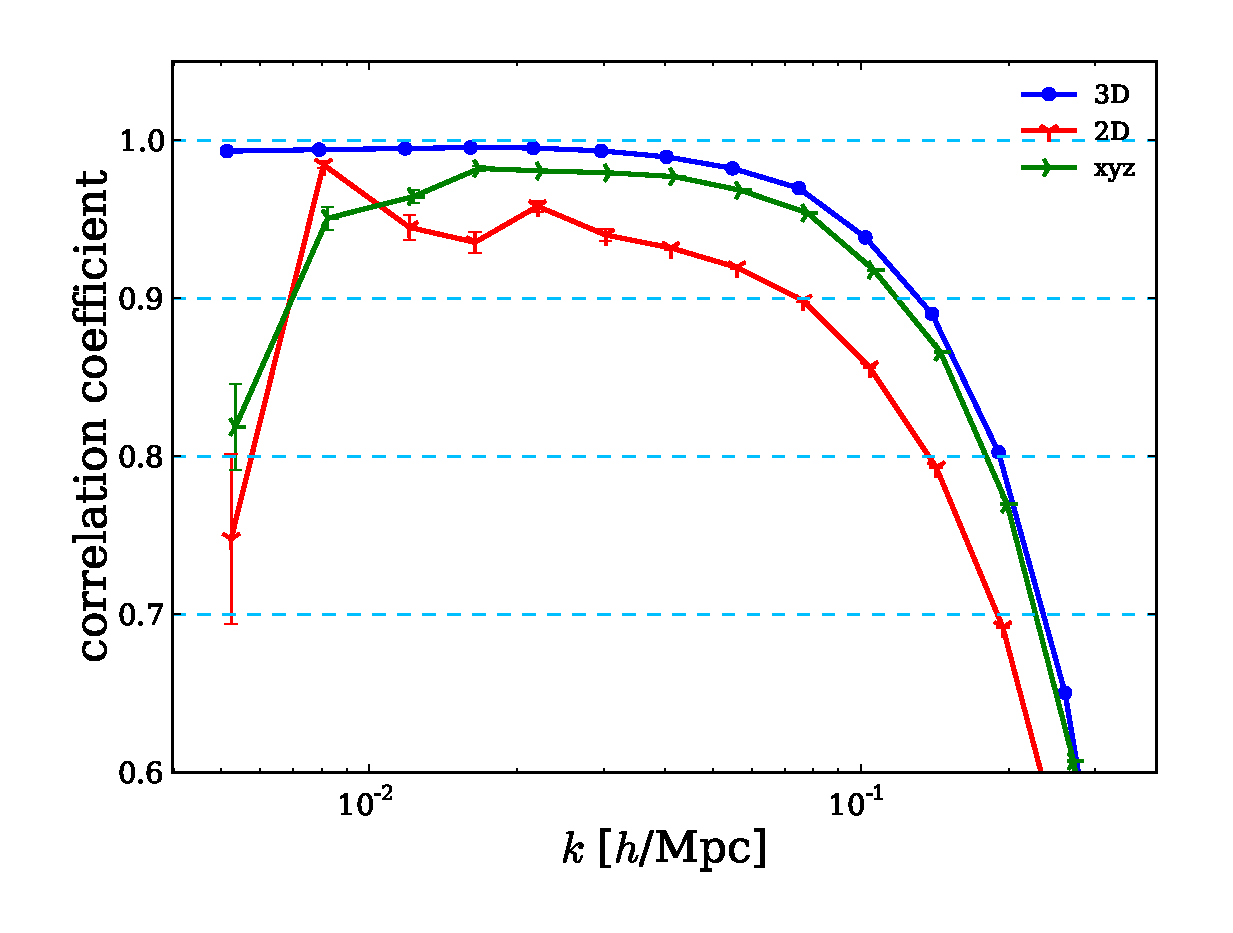
\includegraphics[width=9cm]{1D_correlation_all.eps}
%     \caption{The correlation coefficients (Eq. (\ref{correlation})) from the 2D reconstruction, 3D reconstruction and the reconstruction with $\gamma_{x}$, $\gamma_{y}$ and $\gamma_{z}$.}
%     \label{1Dcorrelation_all}
%\end{figure}

In Fig. \ref{2Dcorrelation} we show the correlation coefficients obtained from three reconstruction methods, which is defined as $P_{\kappa\delta}(k_\perp, k_\parallel)/\sqrt{P_{\kappa}(k_\perp, k_\parallel)P_{\delta}(k_\perp, k_\parallel)}$. We see all the coefficients are better at the lower $k$. Almost at all scales, the correlation coefficients from 3D method are highest, followed by the coefficients from reconstruction with $\gamma_{x}$, $\gamma_{y}$ and $\gamma_{z}$ and the 2D method. In addition, the coefficients from 3D method are isotropic while the results from 2D method are most anisotropic. At larger $k$, the correlation coefficients drop, these can be attributed to the invalidity of our method at small scales. For clearity, we also show the 1D correlation coefficients of the three reconstructions in Fig. \ref{1Dcorrelation_all}. Because of using most fluctuation modes, the 3D reconstruction has the best performance with lowest variance, best stability and highest correlation between the $\kappa$ and the original dark matter field. 

%=======================================

%\subsection{Redshift Space Distortion}\label{section:redshift space distortion}

In the realistic survey, the observed galaxies and halos are shifted from their original position due to the peculiar velocity, resulting in a space with changed structure. For the power spectrum statistics, the redshift space distortion will leave a ``squash'' effect \cite{1987MNRAS.227....1K} at the large scales and a ``fingers of God'' effect \cite{1972MNRAS.156P...1J} at the small scales. For the shear terms of Eq. (\ref{eq10}) that have $\hat{k}_{3}$ term, they will be contaminated by the peculiar velocity anisotropically. 

In order to test how the RSD affects our reconstruction, we perform reconstruction with the dark matter field where the positions of the dark matter particles have been shifted according to the $z$ component of pecular velocities. The position of the dark matter particles in real space $\bm{r}$ is mapped to the position in the redshift space $\bm{s}$ by:
\begin{equation}
\bm{s} = \bm{r} + \frac{(1+z)\bm{v}\cdot\hat{r}}{H(z)}\hat{r},
\label{eq24}
\end{equation}
where $\hat{r}$ is the unit vector along the line of sight and $H(z)$ is the Hubble parameter at the redshift of $z$. Then we carry out the reconstruction again with the 3D method described above. 

\begin{figure}[h!]
      \centering
      %\includegraphics[width=9cm]{1D_correlation_no_rsd.eps}
      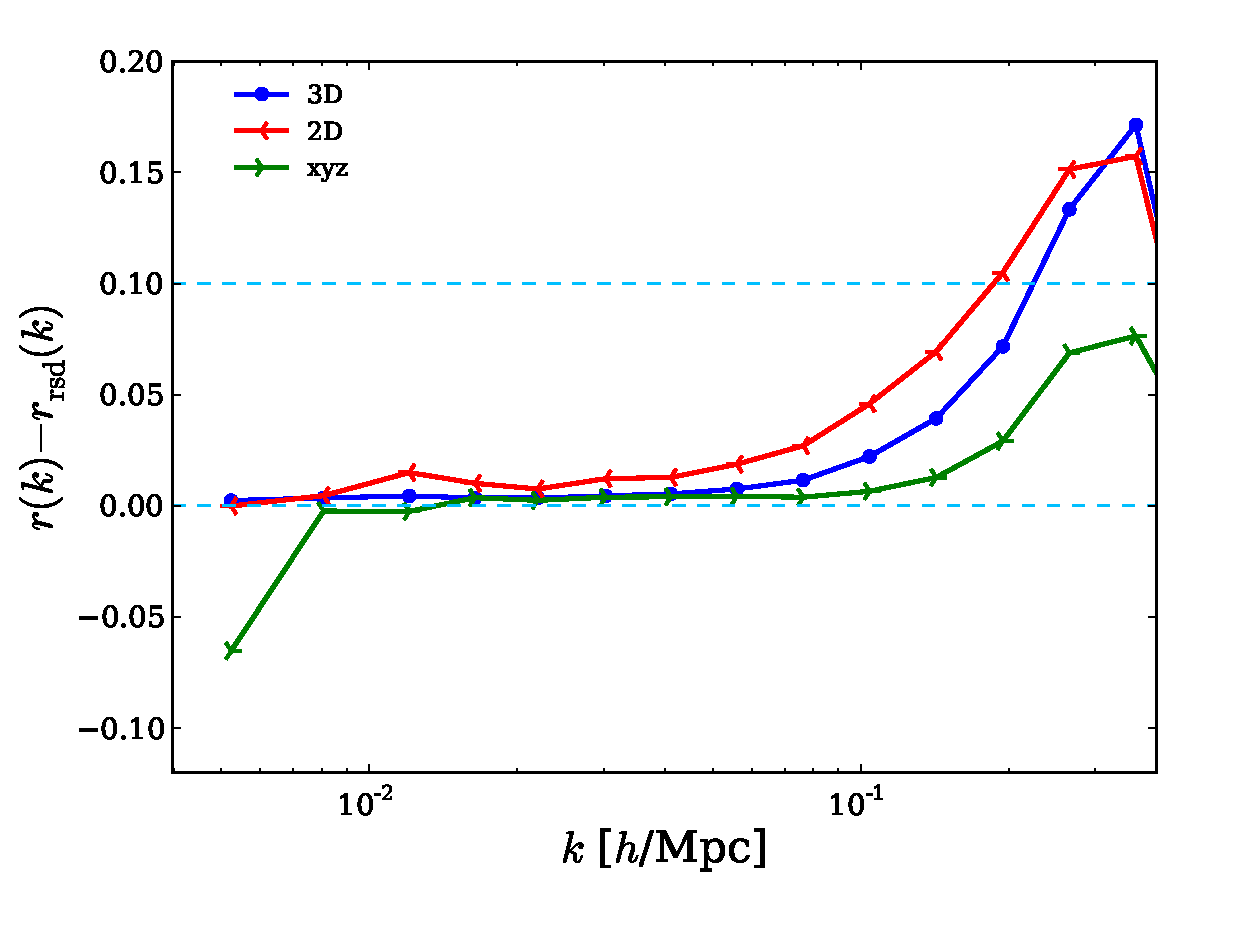
\includegraphics[width=9cm]{1D_correlation_no_rsd_delta.eps}
      \caption{The correlation coefficients from the tidal reconstruction with the original dark matter field and the dark matter field with RSD.}
      \label{1D_correlation_no_rsd}
\end{figure}

RSD effect will change the distribution of the fluctuations and affect the estimators for the tidal shear field which is $\bm{k}$-dependant.  Then, the method described above will be suboptimal when it comes to the reconstruction with a redshift distorted field.
Figure. \ref{1D_correlation_no_rsd} presents the difference of correlation coefficients from tidal reconstructions in different methods with, respectively, original dark matter field and dark matter field with RSD. It shows in all combinations of $\gamma$, the reconstruction with original field have higher correlation. And the 3D method are least influenced by RSD. Combining with the results in Fig. \ref{1Dcorrelation_all}, the 3D method performs best in the reconstruction with the field that is affected by RSD. 

To have the best performance, our estimators should be corrected to account for the RSD effect. However, the influence RSD brings to the reconstructed field becomes obvious only at the small scales, where we do not care about. The little difference at large scales indicates our 3D method is hardly affected by RSD.

%=======================================

\section{Discussion}\label{section:Discussion}
%Our quadratic estimators are established under the gaussian assumption, while there is non-negligible non-Gaussianity buried in the density structure. Under this condition, the Gaussianization of the field becomes an indispensable necessity. Before the reconstruction, a Gaussianization technique is applied to the dark matter field. In principle, the essential solution is to derive a optimal reconstruction method which can be safely applied in the non-Gaussian field, however, this is beyond the scope of this paper and we will investigate the non-Gaussian mothod in the future.

In section. \ref{section:Tidal Reconstruction}, we obtain the estimators for tidal shear fields, however, there may be a bias between the estimators and the real tidal fields. Two reasons may account for this. One of them is the limited coupling modes we make use of when we construct the estimators. This will lead to a misestimation of the interaction between small-scale perturbations and the long-wavelength tidal fields. The other reason goes to the long-wavelength limit could be broke if the long-wavelength tidal shear fields vary fast. This will introduce a $k$-dependent multiplicative bias that gets close to unity when $k$ approaches 0, and decreases and fluctuates as $k$ increases \cite{2008:lu, 2012bucher}. 

Considering the complexity of the nonlinear process, containing the nonlinear modes as many as possible in our algorithm will be much too complicated. In this paper, we directly assume that the nonlinear process only affects the coefficient $f(k,\tau)$ and the change of $f(k,\tau)$ varies slowly in $k$-space. Then the deformation of the local power spectrum, which arises from the distortion under the long-wavelength tidal field is still proportional to $\hat{k}_{i}\hat{k}_{j}t^{(0)}_{ij}$. So, we can correct the bias by deviding the $\kappa$ field by a bias factor. The excellent results of reconstruction prove that our assumption works very well, and there is no need to deduce the estimators by using many high-order coupling modes. 

In addition, the $k$-dependent bias as a consequence of the break of the long-wavelength limit is also absorbed in the bias factor(Eq. (\ref{eq20})), together with the bias resulting from the lack of high-order nonlinear process. We don't have to seperate them apart. From the Fig. \ref{1D_bias_smooth}, we can see the reconstructed density fields from the reconstructions with smoothing nearly have constant biases, while the bias from the reconstruction without smoothing fluctuates. This indicates that the long-wavelength limit holds well if we only use the modes at kind of large scales, which are larger than 1.25 Mpc/$h$ according to the results in Sec. \ref{section:Simulations}. So, we can assume that the $k$-dependant bias to be constant when we model the bias factor. Then these two biases can be corrected together by deviding the $\kappa$ field by a $k$-dependent bias factor.

We also test how RSD affect our reconstruction. The shear terms of Eq. (\ref{eq1}) that have $\hat{k}_{3}$ term will be contaminated by the peculiar velocity. We find that our 3D reconstruction is almost unaffected at the scales where we care about. Deriving the estimators containing the RSD effect, or recovering the dark matter field through ``BAO-reconstruction''\cite{2015arXiv151100663S} will smaller the negative influence from RSD. These beyond the scope of this paper, we leave more detailed analysis of the RSD effect in the future's paper.

%Our reconstruction technique can play an important role in the future cosmology. The reconstruction can be applied to recover the long wavelength modes of the 21cm signal. In the 21cm observational experiments, the long wavelength modes are removed as the results of the foreground subtraction. If the 21cm signal is strongly correlated with the dark matter field and not effected by the ionization fraction and spin temperature, like what happens in the low-z universe, we can reconstruct the long wavelength modes of the 21cm signal with our method, making it possible to correlate with the experiment that only detect the long-wavelength 21cm modes. Besides this, we can measure the redshift-space distortions without sample variance by cross-correlating the reconstructed $\kappa$ field with the original halo field.
%\\\\
%=======================================

\section{Conclusion}\label{section:Conclusion}
In this paper, we update the tidal reconstruction by using all the 5 tidal shear fields. We develop a optimal algorithm of the 3D tidal reconstruction and test this method with simulated dark matter fields. We find that our method can indeed reconstruct the large-scale structure from the small-scale fluctuations in the original density field. The reconstructed density field has an almost unity correlation with the original dark matter field at large scales. Comparing with the reconstructions with other combinations of tidal shear fields, the 3D method performs best with highest correlation, best isotropy and lowest noise. Besides, we find the 3D reconstruction is almost unaffected by the RSD effect. Although some fine details of the reconstruction is needed to be optimized, our 3D method can be an important complement to the tidal reconstruction. 

%=======================================

\section{Acknowledgement}
We acknowledge the support of the Chinese MoST 863 program under Grant No. 2012AA121701, the CAS Science Strategic Priority Research Program XDB09000000, the NSFC under Grant No. 11373030 and 11403071, IAS at Tsinghua University, CHEP at Peking University, and NSERC. The simulations were performed on the BGQ supercomputer at the SciNet HPC Consortium. SciNet is funded by: the Canada Foundation for Innovation under the auspices of Compute Canada; the Government of Ontario; the Ontario Research Fund – Research Excellence; and the University of Toronto.
%=======================================

\bibliographystyle{apsrev}
\bibliography{tide}

\end{document}
